%\iffalse
\let\negmedspace\undefined
\let\negthickspace\undefined
\documentclass[journal,12pt,onecolumn]{IEEEtran}
\usepackage{cite}
\usepackage{amsmath,amssymb,amsfonts,amsthm}
\usepackage{algorithmic}
\usepackage{graphicx}
\usepackage{textcomp}
\usepackage{xcolor}
\usepackage{txfonts}
\usepackage{listings}
\usepackage{enumitem}
\usepackage{mathtools}
\usepackage{gensymb}
\usepackage{comment}
\usepackage[breaklinks=true]{hyperref}
\usepackage{tkz-euclide} 
\usepackage{listings}
\usepackage{gvv}                                        
\def\inputGnumericTable{}                                 
\usepackage[latin1]{inputenc}                                
\usepackage{color}                                            
\usepackage{array}                                            
\usepackage{longtable}                                       
\usepackage{calc}   

\usepackage{multirow}                                         
\usepackage{hhline}
\usepackage{circuitikz}                        
\usepackage{ifthen}                                           
\usepackage{lscape}
\usepackage{tikz}
\newtheorem{theorem}{Theorem}[section]
\newtheorem{problem}{Problem}
\newtheorem{proposition}{Proposition}[section]
\newtheorem{lemma}{Lemma}[section]
\newtheorem{corollary}[theorem]{Corollary}
\newtheorem{example}{Example}[section]
\newtheorem{definition}[problem]{Definition}
\newcommand{\BEQA}{\begin{eqnarray}}
 \newcommand{\EEQA}{\end{eqnarray}}
\newcommand{\define}{\stackrel{\triangle}{=}}
\theoremstyle{remark}
\newtheorem{rem}{Remark}
\begin{document}
 \bibliographystyle{IEEEtran}
 \vspace{3cm}
 \title{\textbf{EC 25}}
 \author{EE23BTECH11048-Ponugumati Venkata Chanakya$^{*}$% <-this % stops a space
 }
 \maketitle

 \bigskip
 \renewcommand{\thefigure}{\theenumi}
 \renewcommand{\thetable}{\theenumi}
 \textbf{QUESTION:}
In the circuit shown, the clock frequency ,i.e.,the frequency of the clock signal,in $12$ kHz. The frequency of the signal at $Q_2$ is $\rule{1cm}{0.15mm}$kHz\\
\begin{center}
\begin{circuitikz}
    % Flip-Flop 1
    \draw (0,0) rectangle (2,3);
    \node at (0.5,2) {$D_1$};
    \node at (1.5,2) {$Q_1$};
    \node at (1.5,1) {$\overline{Q_1}$};
    \draw (-0.5,1) -- ++(0.5,0) node[anchor=west] {CLK};
    %\draw (1,3) -- ++(0,0.5) node[anchor=south] {D1};
    \draw (2,2) -- ++(0.5,0) coordinate (Q1);
    \draw (2,1) -- ++(0.5,0) coordinate (Q1bar);
    
    % Flip-Flop 2
    \draw (4,0) rectangle (6,3);
    \node at (4.5,2) {$D_2$};
    \node at (5.5,2) {$Q_2$};
    \node at (5.5,1) {$\overline{Q_2}$};
    \draw (3.5,1) -- ++(0.5,0) node[anchor=west] {CLK};
    \draw (6,2) -- ++(1.5,0) node[anchor=west] {Q2};
    \draw (6,1) -- ++(0.5,0) coordinate (Q2bar);
    %\draw (5,3) -- ++(0,0.5);

    % OR Gate at (-3,2)
    \node[and port, anchor=in 1] (or1) at (-3,2) {};
    \draw (or1.in 1) -- ++(-0.5,0) ;
    \draw (or1.in 2) -- ++(-0.5,0) ;
    \draw (or1.out) -- ++(0.5,0) |- (0,2);

    % Connections
    %\draw (Q1bar) -- ++(0.5,0) |- (or1.in 1);
    %\draw (Q2bar) -- ++(0.5,0) |- (or1.in 2);
    \draw (Q1) -- ++(0.5,0) -- (4,2);
    \draw (6,1) -- ++(1,0);
    \draw (7,1) -- ++(0,0.8);
    \draw(7,2.2) arc[start angle=90,end angle=270,radius=0.2]; 
    \draw (7,2.2) -- ++(0,1.8);
    \draw (7,4) -- (-4,4) |- (or1.in 2);;
    \draw (-3.5,3.5) -- ++(0,-1.5);
    \draw (2.5,1) -- (2.5,1.8); 
    \draw(2.5,2.2) arc[start angle=90,end angle=270,radius=0.2]; 
    \draw (2.5,2.2) -- (2.5,3.5) -- (-3.5,3.5);
   
    % Clock line
    \draw (3.5,1) -- ++(0,-1.5);
    \draw (-0.5,1) -- ++(0,-1.5);
    \draw (3.5,-0.5) -- (-1.5,-0.5)node[anchor=south] {$12$KHz};
    
\end{circuitikz}
\end{center}
 \solution 
% CLK (Clock signal) diagram
% CLK (Clock) diagram
\begin{center}
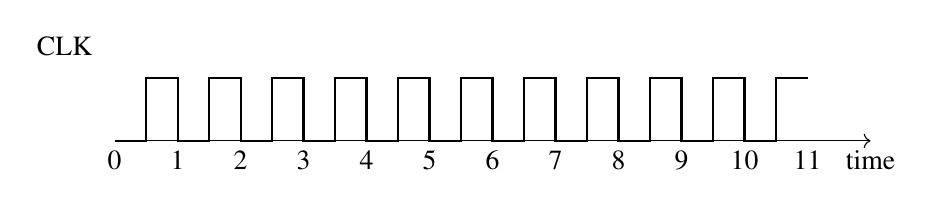
\begin{tikzpicture}[scale=0.8]

% Time axis
\draw[->] (0,-1.5) -- (12,-1.5) node[anchor=north] {time};

% Label the divisions on the time axis
\foreach \x in {0, 1, 2, 3, 4, 5, 6, 7, 8, 9, 10, 11}
    \node[anchor=north] at (\x, -1.5) {\x};

% CLK signal
\draw[thick] (0, -1.5) -- (0.5, -1.5) -- (0.5, -0.5) -- (1, -0.5)
            -- (1, -1.5) -- (1.5, -1.5) -- (1.5, -0.5) -- (2, -0.5)
            -- (2, -1.5) -- (2.5, -1.5) -- (2.5, -0.5) -- (3, -0.5)
            -- (3, -1.5) -- (3.5, -1.5) -- (3.5, -0.5) -- (4, -0.5)
            -- (4, -1.5) -- (4.5, -1.5) -- (4.5, -0.5) -- (5, -0.5)
            -- (5, -1.5) -- (5.5, -1.5) -- (5.5, -0.5) -- (6, -0.5)
            -- (6, -1.5) -- (6.5, -1.5) -- (6.5, -0.5) -- (7, -0.5)
            -- (7, -1.5) -- (7.5, -1.5) -- (7.5, -0.5) -- (8, -0.5)
            -- (8, -1.5) -- (8.5, -1.5) -- (8.5, -0.5) -- (9, -0.5)
            -- (9, -1.5) -- (9.5, -1.5) -- (9.5, -0.5) -- (10, -0.5)
            -- (10, -1.5) -- (10.5, -1.5) -- (10.5, -0.5) -- (11, -0.5);
\node[anchor=east] at (-0.2, 0) {CLK};

\end{tikzpicture}
\end{center}

% D1 (Data Input 1) diagram
\begin{center}
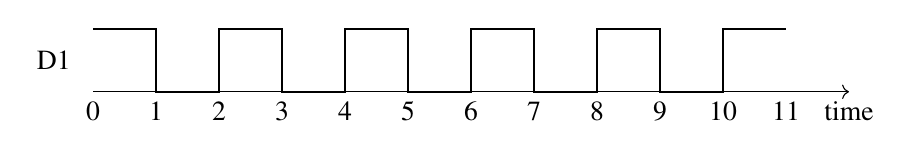
\begin{tikzpicture}[scale=0.8]

% Time axis
\draw[->] (0,-2.5) -- (12,-2.5) node[anchor=north] {time};

% Label the divisions on the time axis
\foreach \x in {0, 1, 2, 3, 4, 5, 6, 7, 8, 9, 10, 11}
    \node[anchor=north] at (\x, -2.5) {\x};

% D1 signal
\draw[thick] (0, -1.5) -- (1, -1.5) -- (1, -2.5) -- (2, -2.5) -- (2, -1.5)
            -- (3, -1.5) -- (3, -2.5) -- (4, -2.5) -- (4, -1.5)
            -- (5, -1.5) -- (5, -2.5) -- (6, -2.5) -- (6, -1.5)
            -- (7, -1.5) -- (7, -2.5) -- (8, -2.5) -- (8, -1.5)
            -- (9, -1.5) -- (9, -2.5) -- (10, -2.5) -- (10, -1.5) -- ++ (1,0);
\node[anchor=east] at (-0.2, -2) {D1};

\end{tikzpicture}
\end{center}

% Q1 (Output of Flip-Flop 1) diagram
\begin{center}
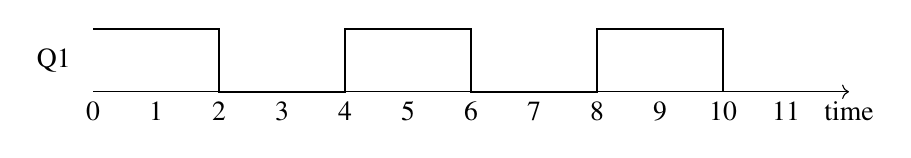
\begin{tikzpicture}[scale=0.8]

% Time axis
\draw[->] (0,-2.5) -- (12,-2.5) node[anchor=north] {time};

% Label the divisions on the time axis
\foreach \x in {0, 1, 2, 3, 4, 5, 6, 7, 8, 9, 10, 11}
    \node[anchor=north] at (\x, -2.5) {\x};

% Q1 signal
\draw[thick] (0, -1.5) -- (2, -1.5) -- (2, -2.5) -- (4, -2.5) -- (4, -1.5)
            -- (6, -1.5) -- (6, -2.5) -- (8, -2.5) -- (8, -1.5)
            -- (10, -1.5) -- (10, -2.5);
\node[anchor=east] at (-0.2, -2) {Q1};

\end{tikzpicture}
\end{center}

% D2 (Data Input 2) diagram
\begin{center}
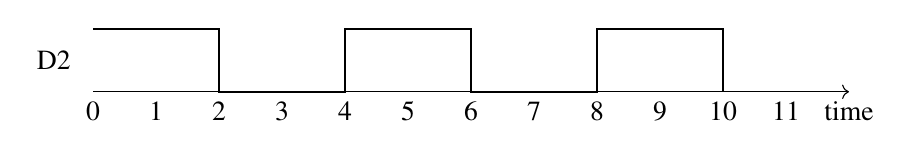
\begin{tikzpicture}[scale=0.8]

% Time axis
\draw[->] (0,-2.5) -- (12,-2.5) node[anchor=north] {time};

% Label the divisions on the time axis
\foreach \x in {0, 1, 2, 3, 4, 5, 6, 7, 8, 9, 10, 11}
    \node[anchor=north] at (\x, -2.5) {\x};

% D2 signal
\draw[thick] (0, -1.5) -- (2, -1.5) -- (2, -2.5) -- (4, -2.5) -- (4, -1.5)
            -- (6, -1.5) -- (6, -2.5) -- (8, -2.5) -- (8, -1.5)
            -- (10, -1.5) -- (10, -2.5);
\node[anchor=east] at (-0.2, -2) {D2};

\end{tikzpicture}
\end{center}

% Q2 (Output of Flip-Flop 2) diagram
\begin{center}
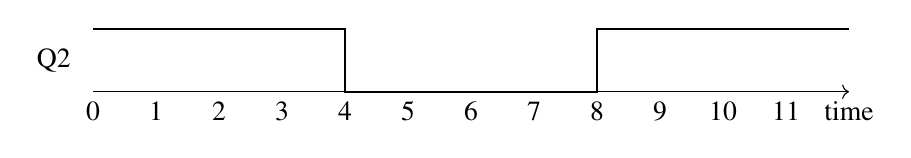
\begin{tikzpicture}[scale=0.8]

% Time axis
\draw[->] (0,-2.5) -- (12,-2.5) node[anchor=north] {time};

% Label the divisions on the time axis
\foreach \x in {0, 1, 2, 3, 4, 5, 6, 7, 8, 9, 10, 11}
    \node[anchor=north] at (\x, -2.5) {\x};

% Q2 signal
\draw[thick] (0, -1.5) -- (4, -1.5) -- (4, -2.5) -- (8, -2.5) -- (8, -1.5)
            -- (12, -1.5);
\node[anchor=east] at (-0.2, -2) {Q2};

\end{tikzpicture}
\end{center}
$\implies $  The frequency of the signal at $Q_2$ is $4$KHz
\end{document}
